%*******************************************************************************
%****************************** Second Chapter *********************************
%*******************************************************************************

\chapter{Related Work}
\label{chapter_related}

\ifpdf
    \graphicspath{{Chapter2/Figs/Raster/}{Chapter2/Figs/PDF/}{Chapter2/Figs/}}
\else
    \graphicspath{{Chapter2/Figs/Vector/}{Chapter2/Figs/}}
\fi

This chapter reviews the related work relevant for this thesis. Since there are many different related work areas that all have their relevance to this thesis, this chapter is divided into different sections dealing with each of them in turn. First section \ref{sec_basicDefinitions} introduces and defines basic the basic terminology that will be used in this thesis. Afterwards section \ref{sec_streamMining} gives a broad overview over the general area of mining data streams but lays a focus on the mining of patterns as well as prediction algorithms, especially for the domain of financial data. Subsequently section \ref{sec_episodes} briefly introduces the concept of episodes and summarizes the related work for episode mining. Finally section \ref{subsec_semanticWeb} concludes with a brief overview over semantic technologies.


\section{Basic Definitions and Terminology}
\label{sec_basicDefinitions}
The basic terminology in this subsection is paraphrased from the event processing glossary created by the Event Processing Technical Society \cite{luckham2011epts}. Note that some of the definitions may be slightly altered or simplified. This is due to the fact that the event processing technical society uses these terms for a very general description of event processing and event processing architectures and thus some original definitions are more complex than what is needed in this thesis. The definitions given here aim to establish a clear terminology for this thesis.

\begin{mydef}
\textbf{Event} An event is either something that is happening in the real world or in the context of computer science an object that represents a real world event and records its properties. The latter can also be referred to as an event object or an event tuple. Note that the term is overloaded, but the context usually gives a clear indication of what is meant.
\end{mydef}

The event processing society argues that the context usually solves the ambiguity in the above definition. Since this may not always be the case I will only use the term \textit{event} in this thesis to refer to event objects unless it is otherwise specified.

\begin{mydef}
\textbf{Simple Event} A simple event is an event that is not viewed as summarizing, representing, or denoting a set of other events. Sometimes this is also referred to as a basic events.
\end{mydef}

These two definitions can sometimes cause confusion. It is important to note that the term event is the most general term, since it can refer to any kind of event, be it simple, derived or complex (see definitions \ref{def_derivedEvent} and \ref{def_complexEvent}). A simple event however is the most basic form of an event and often the ingredient for the creation of more complex events:
Given simple events it is possible to derive events from those or the absence of those. For example the absence of measurement events of a sensor could be used to derive the event of that very same sensor becoming defect. These events are called derived events:

\begin{mydef}
\label{def_derivedEvent}
\textbf{Derived Event} A derived event or synthesized event is an event that is generated according to some method or based on some reasoning process.
\end{mydef}

It is also possible to combine multiple simple events to form what is referred to as complex events:

\begin{mydef}
\label{def_complexEvent}
\textbf{Complex Event} A complex event is a derived event that is created by combining other events. The events can be combined by using certain operators, for example disjunction, conjunction or sequence. An example would be $(A \land B) \rightarrow C$ (event A and B in any order followed by event C).
\end{mydef}

This is a very broad definition of complex events. The choice of allowed operators strongly impacts the expressiveness of complex events. A specific kind of complex events are episodes (see section \ref{sec_episodes}), which will be the main focus of this thesis.
The next notion that needs to be considered is that each individual event normally belongs to a certain class of events, which is referred to as the event type:

\begin{mydef}
\textbf{Event type} The event type, sometimes also referred to as event class, event definition, or event schema is a label that identifies events as members of an event class.
\end{mydef}

Another important term that was not explicitly defined in the event processing glossary, but is very relevant to the topic at hand is the notion of a type alphabet:

\begin{mydef}
\textbf{Type Alphabet} The type alphabet, often simply called the event alphabet, is the set of all possible event types that can occur in the observed system.
\end{mydef}

Event alphabets are often implicitly defined when mining frequent itemsets, patterns or episodes. So far, the different kinds of events have been looked at in isolation without considering the scenario that is most relevant to this thesis which is a stream of events. To do so the notion of timestamps needs to be introduced:

\begin{mydef}
\textbf{Timestamp} A time value of an event indicating its creation or arrival time.
\end{mydef}

Given that an event stream can be defined:

\begin{mydef}
\textbf{Event Stream} An event stream is an ordered sequence of events, usually ordered by the event timings.
\end{mydef}

Note that this rather broad definition of an event stream does not assume anything about the kind of event that is contained in it. A stream can contain very basic forms of events (simple events) but can also be made up out of derived events or even complex events. Also other properties, for example that the stream is constantly updating (new events coming in), are not considered yet.


\section{Data Stream Mining}
\label{sec_streamMining}
As already mentioned in the introduction data streams present a challenge to data miners in many ways. This section aims to both give a general overview over the broad research area of mining data stream as well as specifically cover the related topics of pattern mining and prediction (forecasting). \\

\subsection{Taxonomy of the Research Areas}
First of all it is useful to note that many research areas in classical data mining are also of interest when processing streams. However, data streams impose severe restrictions on the algorithms, such as them having to use only one pass over the data and that they should be incremental. Most data mining algorithms for the classical scenario, in which the underlying data is a static database, do not satisfy these properties. Thus the algorithms need to be modified and often approximations have to be made. A comprehensive, basic overview over the application of different data mining tasks and how they can be applied to streams was comprised by Gaber et al. \cite{gaber2005mining}. Note that the paper by Gaber et al. was published in 2005, so quite a lot of work has been done since then, which means that these papers are obviously not present in their literature review. However the overview provided by the authors is still very useful, since it brings structure to the large field of data stream mining. A taxonomy that follows the basic structure of the paper by Gaber et al. is visualized in figure \ref{fig_streamMiningTaxonomy}.

\begin{figure}[h]
	\centering
  	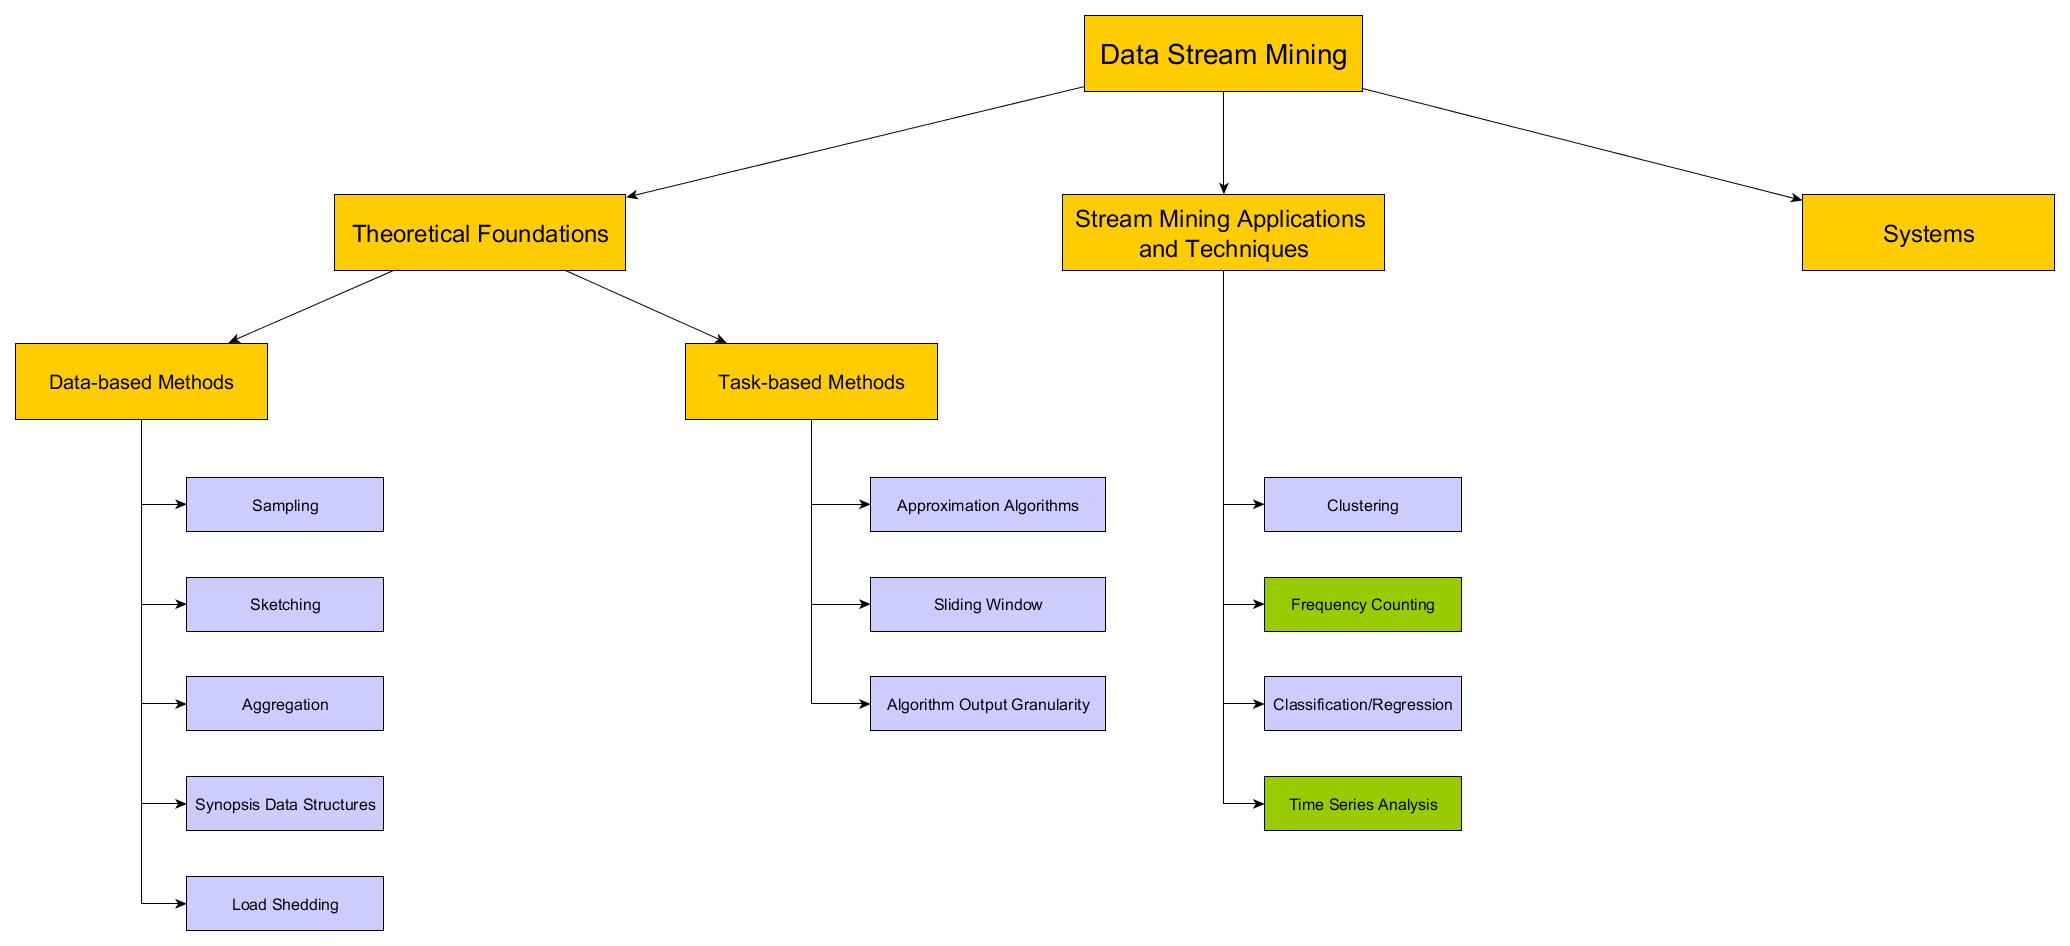
\includegraphics[width=\textwidth]{streamMiningTaxonomy}
	\caption{A taxonomy of the research areas of data stream mining.}
	\label{fig_streamMiningTaxonomy}
\end{figure}

Figure \ref{fig_streamMiningTaxonomy} shows that the state of the art in data stream mining can be roughly divided into three basic parts: Theoretical Foundations, Mining Techniques and Applications as well as Systems. The theoretical foundations deal with general approaches on how to deal with the issues of data streams. Some notable techniques are sampling \cite{manku1999random}, the usage of synposis data structures or approximation algorithms like the lossy counting algorithm \cite{manku2002approximate} as well as the focus on the most recent events by using sliding windows \cite{gama2010knowledge}, which are incrementally updated.\\
The second category contains the actual mining techniques and applications, which are well known from classical data mining. Most relevant to this thesis are the research areas of pattern mining algorithms, prediction strategies and time series analysis. Since the latter two research areas are closely linked to each other, they will be discussed in the same subsection.
The last category in the taxonomy is less focused on research issues and conceptual or algorithmic problems but instead lists the existing data stream processing systems (to that date). Since that is less relevant to this thesis, existing systems are not further discussed.

\subsection{Pattern Mining in Data Streams}
\label{subsec_PatternMining}
One of the first popular use cases of pattern mining in static databases was the mining of frequent itemsets and association rules. The problem of frequent itemset mining is that if given a set of items $I = \{I_1,...,I_n\}$ and a database containing subsets (also called transactions) of $I$ one aims to determine which subsets of the items occur frequently together. The first efficient solution to this problem was introduced by Agrawal et et al. \cite{agrawal1993mining}. Since then techniques for static databases have evolved. Different approaches, such as candidate generation or pattern growth strategies are nicely summarized in a paper by Han et al. \cite{han2007frequent}. Adapting pattern mining approaches to data streams presents the challenges of limited memory and that the frequency of patterns changes over time. The groundwork for a lot of algorithms was laid by a paper suggesting two approximation algorithms to maintain approximate frequencies: the sticky sampling and the lossy counting algorithm \cite{manku2002approximate}. Originally these algorithms were used to maintain the frequency of single items, but the algorithms can be generalized to work for frequent itemsets, too. A slightly different approach was chosen by Gianella et al. who have developed an algorithm to incrementally maintain approximately frequent itemsets for the most recent time windows using tilted time window frames \cite{giannella2003mining}. Another different approach is to mine the exact set of frequent itemsets, but only maintain the most recently frequent ones \citep{tanbeer2009sliding}. The authors of this paper use a sliding window and tree-restructuring algorithms to achieve this goal. This work is extended by Lee et al. by focussing on maximal patterns \cite{lee2014sliding}. \\
It is important to keep in mind that mining frequent itemsets is just a subarea of the much more general field of pattern mining. Mining interesting or frequent patterns can be done in many different data representations, such as sequences \cite{mendes2008stream} or graphs \cite{bifet2011mining}. Approaches are often similar, but differ in details. The patterns that will be focused on in this thesis are episodes. It should be noted that authors of papers concerned with episode mining sometimes use the terms \textit{data stream} and \textit{sequence} interchangeably, since they refer to data streams but then use algorithms that require multiple passes over the data, which is only possible if given static sequences. Since episode mining is a core topic of this thesis, it is dealt with exclusively in section \ref{sec_episodes}.

%\subsection{Complex Event Processing and Episode Mining}
%\label{subsec_eventProcessing}
%Before talking about the state of the art in complex event processing it is first important to clarify the term \textit{"event"} which is a is very broad term that is used in many different areas of science. Even when restricted to computer science there may be different definitions with subtle differences. As already explained in the introduction this thesis will focus on events as defined by the glossary of the event processing society \cite{luckham2011epts}.
%When talking about processing complex events there is an important difference between two cases:
%
%\begin{itemize}
%	\item The patterns of interest are known before looking at the data. This is called complex event detection.
%	\item There is no prior knowledge about which patterns might be interesting, they need to be discovered while looking at the data. This is called complex event discovery or complex event mining (which basically means that data mining methods need to be employed)
%\end{itemize}
%
%Complex event detection usually revolves around specification and query languages for complex events \cite{eckert2009complex}. Quite a few different specification and query languages have been developed, such as SNOOP \cite{chakravarthy1994snoop} or the SASE event processing language \cite{wu2006high}. \newline
%Discovering interesting complex events of arbitrary structure in data streams is a very challenging task, thus most work focuses on specific types of complex events. A popular example is mining frequent sequences of events (basically complex events that only use the sequence operator) \cite{bettini1998mining} \cite{hasan2015probabilistic}. \newline
%This thesis deals with a more expressive type of complex events: Episodes. Originally episodes were researched without any relation to event processing \cite{mannila1995discovering}. 
%Episodes have roughly been categorized as serial, parrallel or composite and there are different mining methods proposed for each of these \cite{mannila1995discovering} \cite{zhou2010mining}. The connection between episodes and hidden markov models was also explored in a PHD thesis by Laxman \cite{laxman2006discovering}.
%Evaluating episode mining algorithms on real-life datasets is often difficult due to a lack of knowledge about the ground truth. Thus, generation of realistic, synthetic datasets has been looked into as well \cite{zimmermann2012generating}.




\subsection{Prediction and Time Series Analysis in Data Streams}
\label{subsec_timeSeriesAnalysis}

Before reviewing the related work it is important to distinguish time series from data streams. Both concepts are similar and also have overlapping research areas. A time series refers to a temporally ordered sequence of data points. Usually time series contain numerical values, examples of such data are:

\begin{itemize}
	\item values of a stock market index over a trading day
	\item measurement values sampled from continuous readings of a temperature sensor
	\item electrocardiography readings of a human heart
\end{itemize}

Data streams are also ordered sequences of data. The important distinctions between time series and data streams are: 

\begin{itemize}
	\item Data streams continuously have new data points coming in, thus are continuously growing. This does not have to be the case for time series data. A database that records electrocardiography readings of different patients still contains time series data, however these are not data streams, since the readings are finished and no longer updating.
	\item In contrast to time series it is not uncommon in data streams to have streams of categorical values or events, whereas values of time series are usually numeric.
\end{itemize}


The combination of both, a time series data stream, is a time series that is constantly updating, for example an electrocardiography reading that is currently taking place, or stock values that are being recorded over a day. In these cases the time series must be processed online. \newline
The research area of (online) time series analysis is rather broad, meaning there are a variety of different objectives that can be of interest when analyzing time series. Thus it is helpful to first get an overview over the most common objectives and techniques in a similar way as the taxonomy for data stream mining visualized in figure \ref{fig_streamMiningTaxonomy}. The main source for this subsection is the book by J. Gama \cite{gama2010knowledge}. Figure \ref{fig_timeSeriesInDataStreamsOverview} visualizes the different areas of interest in time series analysis in data streams mentioned by the author.

\begin{figure}[h]
	\centering
  	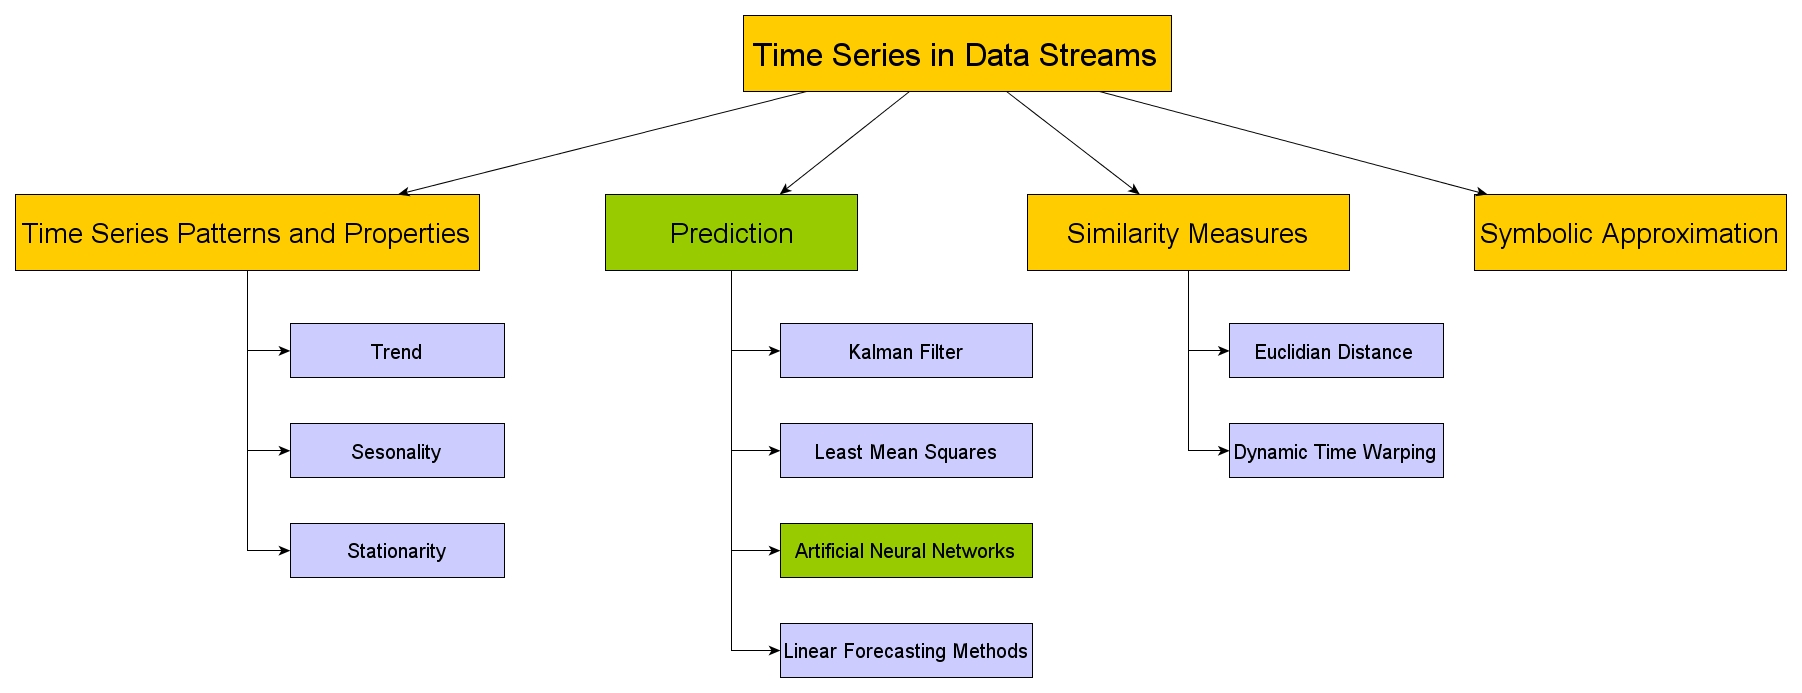
\includegraphics[width=\textwidth]{timeSeriesInDataStreamsOverview}
	\caption{An overview over the different research areas in time series analysis in data streams. The subcategory \textit{"Prediction"} is marked green, since it is of special interest in this thesis and thus will be discussed extensively.}
	\label{fig_timeSeriesInDataStreamsOverview}
\end{figure}

Note that the research area of time series analysis is large and therefore there are important subareas that are not mentioned by the author. Examples of such research areas are curve fitting, function approximation and time series segmentation. The most relevant subtopic of time series analysis for this thesis is prediction. Prediction (also called forecasting) in data streams or time series can done via classification \cite{leung2000forecasting} or regression methods \cite{alzghoul2012data}. Classification refers to a problem in machine learning in which objects are to be identified and assigned to a certain class (for example if given data about a flower, determine its species). Models that solve these problems are also called classifiers. Regression is a similar problem, except that instead of assigning categorical values to objects, the goal is now to predict numerical values (for example if given data about an animal, determine its exact age). \\
When applying classifiers to data streams there is an additional challenge to the time and memory constraints, which is called concept drift. The term of concept drift refers to the fact that the underlying class distribution may change, which will make the originally built model invalid over time. In order to address this problem classifiers need to be restructured in an online learning process \cite{wang2003mining}. \\
Forecasting methods based on regression can be divided into linear and non-linear methods. Linear models are usually simpler, but are at a disadvantage when the underlying model is non-linear \cite{zhang2003time}. Non-linear methods, such as neural networks are more powerful, in fact it has been shown that neural networks can in theory model any non-linear function \cite{abraham2005artificial} \cite{funahashi1989approximate}. However, building and training an actual neural network is a difficult task, since multiple design choices (such as the number of hidden neurons, the activation function and the initial weights) need to be made, which usually requires expert knowledge of both the underlying domain as well as neural networks in general in order to train an appropriate network \cite{abraham2005artificial}. Researchers have also tried to combine both approaches in order to form hybrid methods \cite{zhang2003time}. \newline
Neural networks were originally conceived as batch methods, meaning they were used in an offline scenario with no new data coming in constantly. However adapting them to the stream environment is surprisingly simple in most cases and has been done on multiple occasions \cite{chang2002real} \cite{frank2001time}. In fact, the streaming environment can be beneficial to neural network training, since training a neural network in a static environment usually means making multiple passes over the training data, due to the lack of training data. If done incorrectly this can result in overlearning the training data and thus poor generalization. In the streaming environment however, there is an abundance of data, which means that each example has to be processed only once \cite{gama2010knowledge}. \newline
Predicting or forecasting time series values is normally very domain specific which results in different domains having their own specialized forecasting methods or specific modifications of popular predictive models. Some of the domains in which time series forecasting is relevant are:

\begin{itemize}
	\item Forecasting the electricity demands of households \cite{veit2014household}
	\item Forecasting the power output of solar energy plants \cite{inman2013solar}
	\item Forecasting natural disasters such as droughts \cite{mishra2006drought}.
	\item Forecasting price developments in stock markets.
\end{itemize}

The last domain is especially relevant to this thesis, since the dataset used in the evaluation comes from this domain. It is therefore necessary to take a more extensive look at the specific domain of financial time series forecasting. It is important to note that in a lot of cases, financial time series are not analyzed in a streaming environment. Authors commonly attempt to forecast daily closing values of stock markets, which means that in this case data velocity is very low (one new data point per day). However many techniques applied in these scenarios can also be applied in more rapidly moving streams. Examples of these are autoregressive models \cite{terasvirta1994specification} or artificial neural networks \cite{gama2010knowledge}. \newline
A good starting point into the prediction of stock market movements is provided by a literature study by Atsalakis et al. \cite{atsalakis2009surveying}. The authors review more than 100 papers that attempt to predict stocks or stock indices. Figure \ref{fig_financialTimeSeriesPredictionOverview} visualizes some of the different properties and experimental settings of the approaches covered by Atsalakis et al.

\begin{figure}[h]
	\centering
  	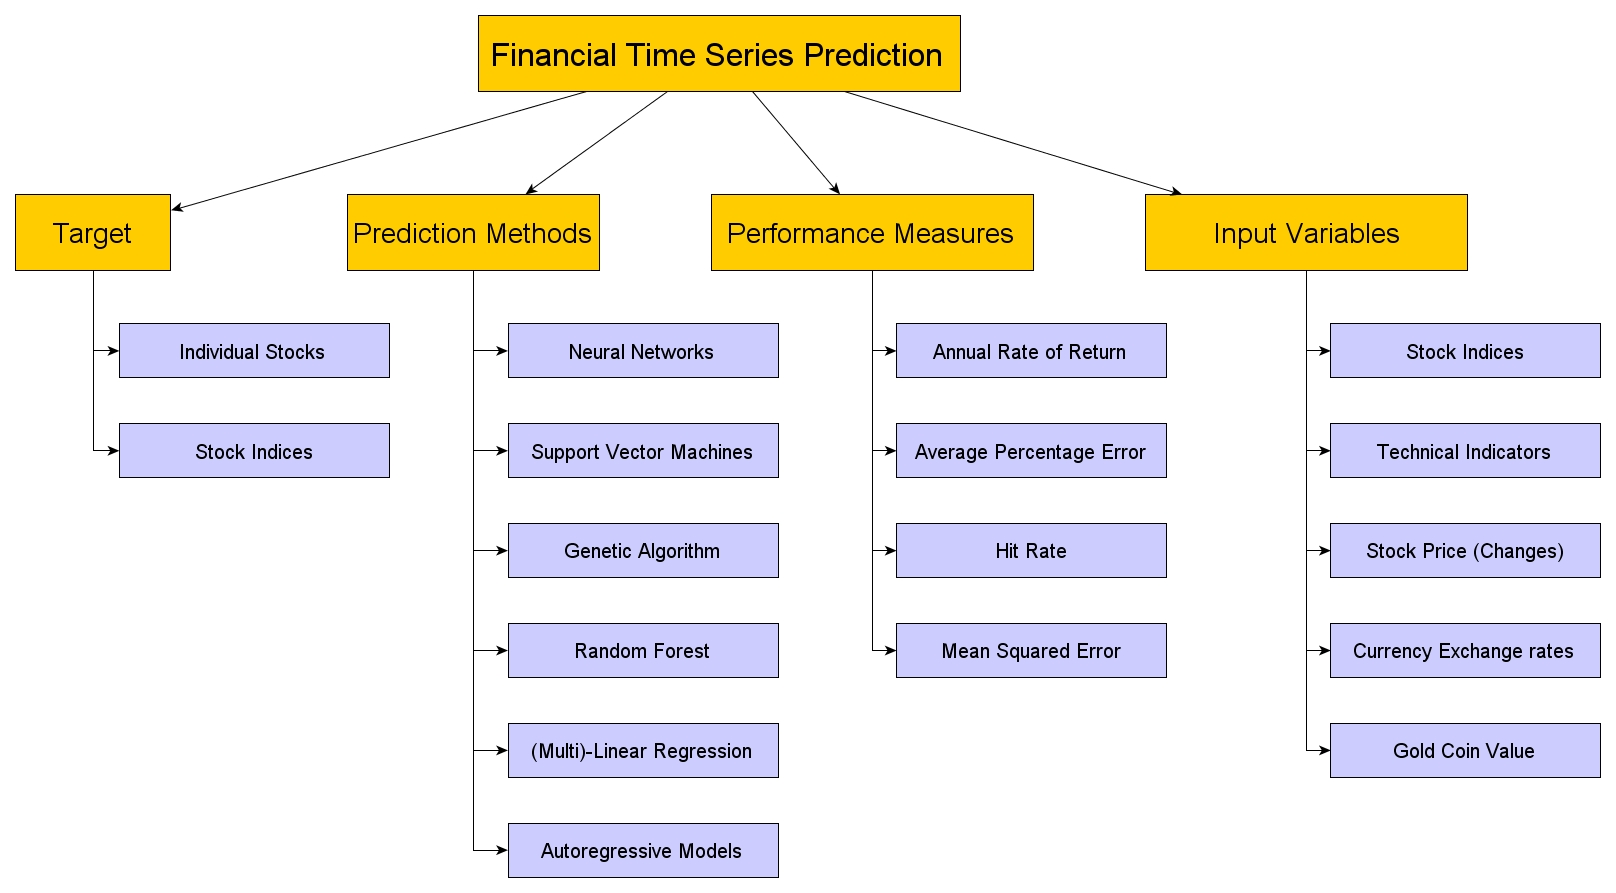
\includegraphics[width=\textwidth]{financialTimeSeriesPredictionOverview}
	\caption{An overview over different properties, experimental settings and approaches to the forecasting of of stock markets}
	\label{fig_financialTimeSeriesPredictionOverview}
\end{figure}

Most of the visualized information in figure \ref{fig_financialTimeSeriesPredictionOverview} was taken from the previously mentioned literature study by Atsalakis et al. \cite{atsalakis2009surveying}. However  some pieces of work were not covered in that study, for example a comparative study of different models including the otherwise rarely used random forest \cite{kumar2006forecasting}. The different properties and categories visualized in figure \ref{fig_financialTimeSeriesPredictionOverview} are briefly reviewed:

\begin{itemize}
	\item \textbf{Target:} The target that is to predict can in theory be any financial index, indicator or price of interst. Many researchers tried to forecast the movement of stock indices \cite{zhang2009stock} \cite{van2001financial} \cite{kumar2006forecasting} . However, also individual stocks have received attention \cite{mahfoud1996financial}. 
	\item \textbf{Performance Measures:} When building models it is crucial to measure their performance to enable comparison to other models. The number of different performance measures in this case is surprisingly large and diverse. The employed measures range from economic measures, such as the annual rate of return or the Hit-Rate to more technical measures such as the average percentage error or the mean squared error to only name a few. It is impractical to visualize or enumerate all measures that are in use. For a comprehensive list I refer the reader to the literature study by Atsalakis et al. \cite{atsalakis2009surveying}.
	\item \textbf{Input Variables:} This is probably the most important category. No matter which kind of elaborate model is built, if the choice of the input variables is poor, meaning they contain little information, then the model built from those simply can not perform well. This is especially true for financial time series, since those are known to be chaotic and noisy \cite{zhang2009stock}. In fact there are researchers that argue that financial time series follow the principle of random walks, which would imply that achieveing better than random accuracy when forecasting financial time series based on historical data is impossible \cite{fama1965behavior}. However there is a considerable amount of papers that suggest otherwise, since accurate prediction results have been achieved by multiple authors based on multiple different forecasting methods (see the literature study by Atsalakis et al. for examples \cite{atsalakis2009surveying} ). Input variables for stock market prediction usually include historical stock data. Other financial indicators such as stock indices, gold price or currency exchange rates. are also commonly used.
	\item \textbf{Prediction Methods:} While figure \ref{fig_financialTimeSeriesPredictionOverview} mentions many different approaches to the forecasting of stock markets, a large majority of the published papers in this area uses some form of neural network. In fact Atsalakis et al. note that 60\% of the papers they surveyed use feed forward Neural Networks and recurrent networks \cite{atsalakis2009surveying}. 
\end{itemize}

Most of these models have in common that they are highly specialized and take considerable effort to build and train, which means that it can be difficult to use them in a different environment (for example with a different amount of data, slightly different input variables, etc...).

\section{Episode Mining}
\label{sec_episodes}
This thesis deals with a specific type of complex events called episodes. Despite being a rather specialized area of research there exists quite a bit of related work that deals with episode mining. What is notable is that there are some discrepancies in terminology. Different authors sometimes use different terms to refer to the same concept or use the same term but with  a different meaning. These discrepancies will be mentioned here and the exact definitions for this paper will be given in chapter \ref{chapter_background}. \\
Before diving into the previous work on episodes it is important to have a rough idea of what kind of patterns episodes are. Thus a short and informal explanation is presented here, whereas chapter \ref{chapter_background} will give a much more detailed and formal definition of all concepts revolving around episodes. \\
Most simply put, episode patterns are partially ordered sequences of events. They can be visualized as directed acyclic graphs like the example episode shown in figure \ref{fig_exampleCompositeEpisode}. 

\begin{figure}[h]
	\centering
  	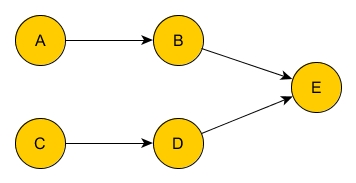
\includegraphics[width=.4\textwidth]{exampleCompositeEpisode}
	\caption{An example episode pattern visualized as a directed acyclic graph. This example pattern specifies that event $A$ and event $C$ may occur in any order, however $A$ must come before $B$ and $C$ must come before $D$, $E$ must occur last.}
	\label{fig_exampleCompositeEpisode}
\end{figure}

Episodes are usually mined from a very large sequence. This distinguishes the concept of episode mining from the concept of sequential pattern mining, which takes place on a sequential database, in which there are many records and each record is a sequence of events \cite{wu2013mining}.
The research concerning episodes can be organized in basic categories as visualized in figure \ref{fig_episodeOverview}.

\begin{figure}[h]
	\centering
  	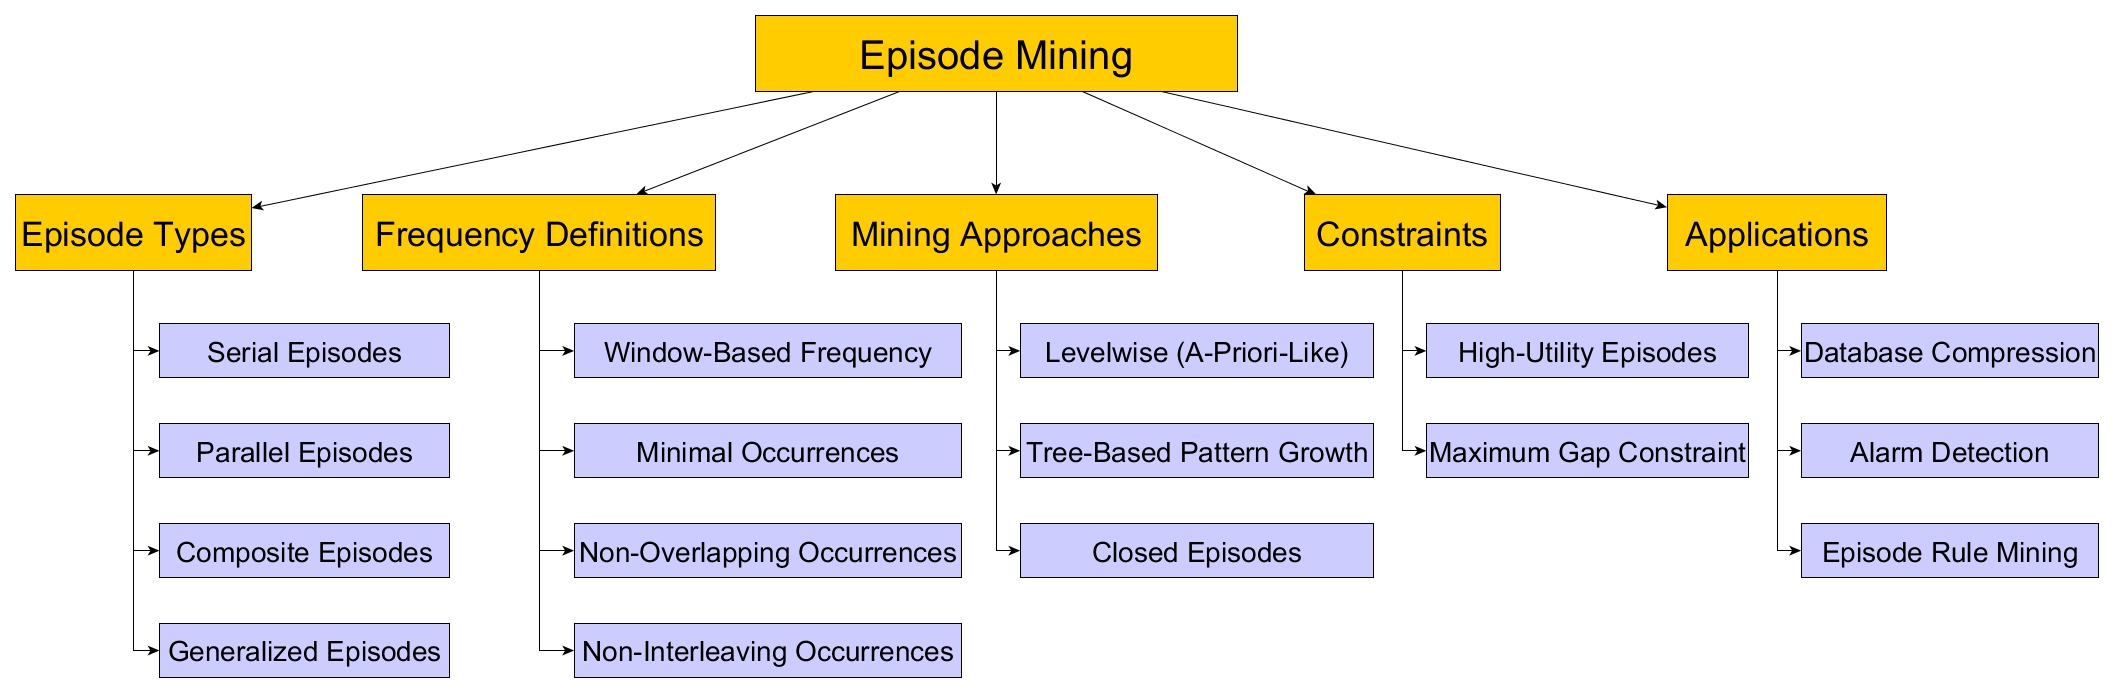
\includegraphics[width=\textwidth]{episodeOverview}
	\caption{A rough categorization of the existing research in episode mining}
	\label{fig_episodeOverview}
\end{figure}

The different types of episodes that have been looked at in the literature are mostly special cases of general episodes. Mannila et al. introduced the three concepts of serial, parallel and composite episodes \cite{mannila1995discovering}. According to their definitions serial episodes are episodes that have a total ordering (essentially sequences), parallel episodes are episodes without any order (essentially multisets) and composite episodes are episodes that have some order imposed on the events, but do not need to have a total ordering (like serial episodes do). There are however altering definitions of composite episodes in the literature, for example both Bathoorn et al. \cite{bathoorn2007finding} and Baumgarten et al. \cite{baumgarten2003tree} deviate from the original definition and redefine composite episodes as sequences of sets. Section \ref{sec_basicEpisodeDefinitions} explains the difference between the two definitions in more detail. A fourth type of episode are generalized episodes which have been investigated by S. Laxman in his PHD thesis \cite{laxman2006discovering}. The main difference between classic episodes and generalized episodes is that classic episodes assume that the basic events are instantaneous, whereas generalized episodes can be mined from events that have a duration. It is notable that most work focuses on serial and parallel episodes \cite{mannila1995discovering} \cite{mannila1997discovery} \cite{laxman2006discovering} \cite{laxman2007fast}. Authors have already identified this gap in the research and have come up with two different reasons:
\begin{enumerate}
	\item The problem of frequent pattern explosion is already significant for serial and parallel episodes, but still much worse for composite episodes \cite{bathoorn2007finding}.
	\item Detection of composite episodes (checking whether a given composite episode occurs in a sequence) is NP-complete, since 3-SAT can be reduced to this problem \cite{tatti2011mining}.
\end{enumerate}

An exception is a paper by Achar et al. which introduces an algorithm to mine injective episodes with general partial orders \cite{achar2012discovering}. However the authors still require the episodes to be injective (each event type occurs only once). \\
When mining frequent episodes from sequences, frequency of episodes can be defined in multiple ways. Since the different variants of episode frequency need to be carefully considered in this thesis I do not give a brief overview here but instead devote several sections of chapter \ref{chapter_background} to discuss the different frequency definitions. Specifically section \ref{sec_windowBased} gives a detailed explanation of the window based frequency, whereas section \ref{sec_otherFrequency} provides an overview over the other frequency definitions that have been used in the literature. \\
The different mining approaches for episodes are similar to well known approaches for frequent itemset mining. Since most episode frequency definitions follow the apriori principle, a level-wise approach like in frequent itemset mining \cite{agrawal1993mining} is suggested by many authors \cite{mannila1995discovering} \cite{laxman2006discovering}. As an alternative, tree growth methods have been proposed, in which candidate episodes are represented in a tree data structure that gets grown as the algorithm progresses \cite{baumgarten2003tree}. Since frequent pattern explosion is an issue when mining frequent episodes it is unsurprising that the concept of closed patterns from classical pattern mining \cite{wang2003closet+} has been adapted to episodes \cite{zhou2010mining} \cite{tatti2011mining}. \\
When mining episodes, authors have considered several constraints or specific scenarios. Usually one is interested to mine episodes that are local, meaning the events of the episode are supposed to happen close to each other (time-wise). The maximum duration of an episode can be restrictd in different ways, for example by specifying a window size \cite{mannila1995discovering}, when employing the window-based frequency or by a maximum gap constraint, which restricts the maximum time difference between two events of an episode \cite{meger2004constraint}. Another special scenario that considers external constraints is the mining of high-utility episodes, in which one is not interested in frequent episodes but instead into those episodes that cover events that have a high utility score (which is given externally) \cite{wu2013mining}. \\
Mining episodes from data streams has received attention recently for example by Ao et al. \cite{ao2015online}, who developed an online mining algorithm for the most recently frequent serial episodes. The similar problem of mining the most recent top-k episodes has also received attention \cite{patnaik2012efficient}.\\
The applications for episode mining are diverse and some of them are mentioned in the following.

\begin{itemize}
	\item Mannila et al. (arguably the researchers to make episode mining a popular task) were motivated to mine episodes in order to analyze alarms in telecommunication systems \cite{mannila1997discovery}.
	\item Several authors attempt to describe, summarize or compress databases or large sequences by mining appropriate episodes. Examples of research in this application area include the work by Bathoorn et al. \cite{bathoorn2007finding} as well as the work by Vreeken et al. \cite{vreeken2012summarising}.
	\item Episode mining has been used to extract rules from sequences in several different domains, such as geophysics (finding dependencies between earthquakes) \cite{meger2004constraint} or health care (analysis of temoral dependencies between risk factors for atherosclerosis) \cite{meger2004mining}.
	\item Finally, episode mining has been used to build predictive models. Laxman et al. describe in their paper how they mine serial episodes to learn hidden markov models to predict events in sequences \cite{laxman2008stream}. 
\end{itemize}

\section{Semantic Technologies}
\label{subsec_semanticWeb}
Semantic technologies in general are based around the idea to annotate data with meaning in order to enable algorithms to make better decisions and reason about the data. The research area of semantic technologies became popular with an article by Berners-Lee et al. in 2001 in which the authors presented their vision of the semantic web \cite{berners2001semantic}. An article explaining the basic ideas and technologies that also reviews some progress that was made was published by Shadbolt et al. in 2006 \cite{shadbolt2006semantic}. In order to assign meaning to data, the domain of the data needs to be understood, categorized, annotated and structured. Such a structured representation of domain knowledge is called an ontology \cite{noy2004semantic}. Ontologies are made for many different domains, such as linguistics and natural language processing \cite{dahlgren1995linguistic}, genetics \cite{botstein2000gene} or the financial industry \cite{bennett2014adopting}. Ontologies are commonly formalized using the Web Ontology Language \cite{bechhofer2009owl}, however domain knowledge can take many forms which leads to research on approaches to automatically learn ontologies from various sources \cite{maedche2012ontology} \cite{ijntema2012lexico}. \\
Integrating semantic knowledge into data mining processes \cite{mabroukeh2009using} or mining semantic data itself \cite{stumme2006semantic} are challenging research areas. A very broad overview on how data mining and machine learning techniques can be applied to semantic data sources was comprised by Rettinger et al. \cite{rettinger2012mining}. One common issue with semantic knowledge and ontologies that was also identified by Retting et al. is that real world ontologies are usually either very detailed in terms of the formal schema or contain a large amount of concrete data but rarely both. Having a detailed ontology is helpful in order to understand the domain, however in order to use the semantic knowledge one requires concrete data about specific entities. Concrete semantic data is commonly expressed using the Resource Description Framework (RDF) \cite{miller1998introduction}. One of the largest and most well known semantic databases is the DBpedia, which contains data extracted from structured information in wikipedia articles \cite{auer2007dbpedia}. The DBpedia can be queried using SPARQL, a query language for RDF-data \cite{perez2006semantics}. With these tools in hand it is possible to identify concepts or entities and query the DBpedia for additional semantic knowledge linked to entities of interest.


%\section*{Subplots}
%I can cite Wall-E (see Fig.~\ref{fig:WallE}) and Minions in despicable me (Fig.~\ref{fig:Minnion}) or I can cite the whole figure as Fig.~\ref{fig:animations}


%\begin{figure}
%  \centering
%  \begin{subfigure}[b]{0.3\textwidth}
%   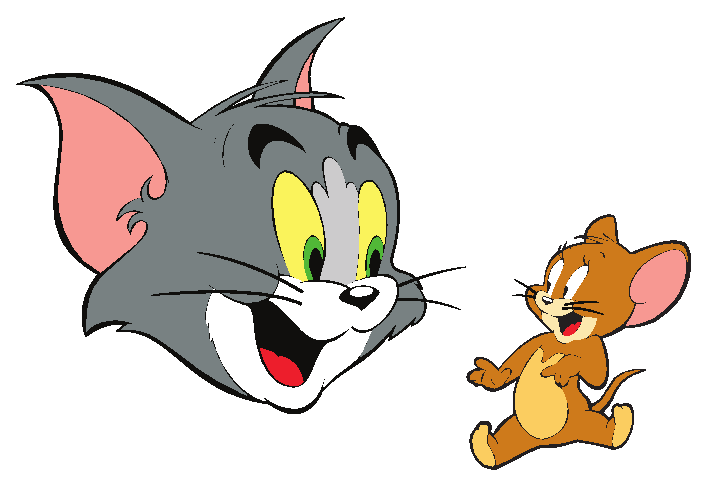
\includegraphics[width=\textwidth]{TomandJerry}
%  \caption{Tom and Jerry}
%    \label{fig:TomJerry}   
%  \end{subfigure}             
%  \begin{subfigure}[b]{0.3\textwidth}
%    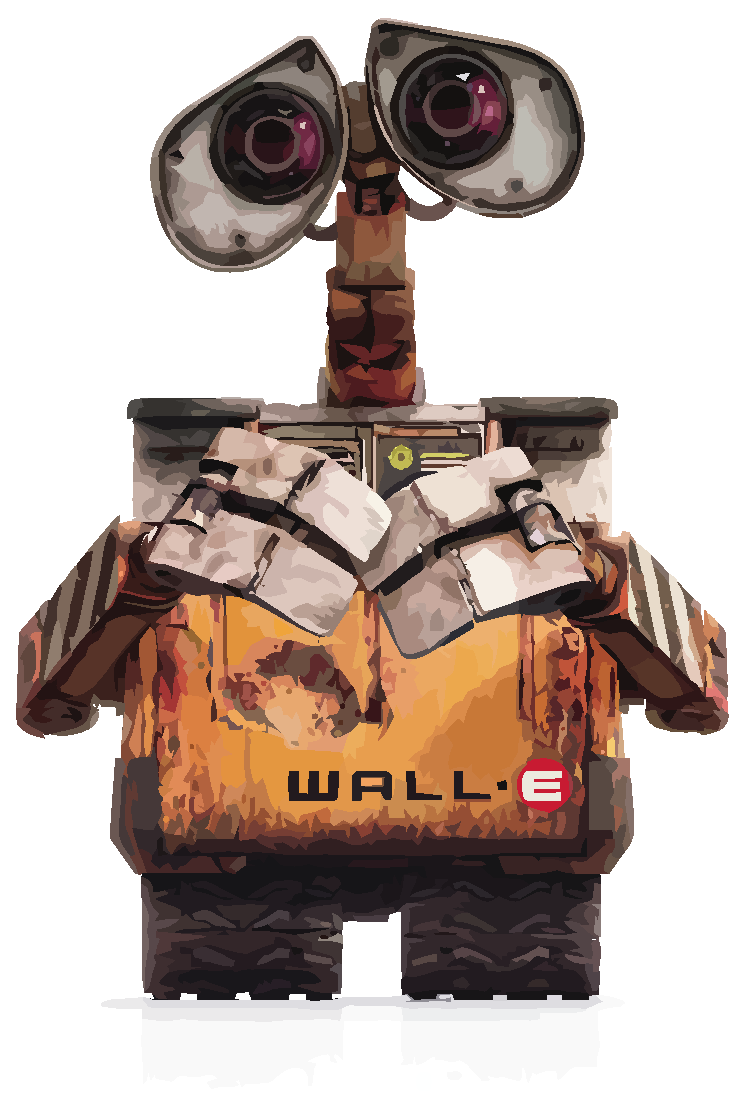
\includegraphics[width=\textwidth]{WallE}
%    \caption{Wall-E}
%    \label{fig:WallE}
%  \end{subfigure}             
%  \begin{subfigure}[b]{0.3\textwidth}
%    
\includegraphics[width=\textwidth]{minion}
%    \caption{Minions}
%    \label{fig:Minnion}
%  \end{subfigure}
%  \caption{Best Animations}
%  \label{fig:animations}
%\end{figure}


